\section{Findings and Discussions}  \label{sec:discussion}
This section presents the experimental findings listed by research question: RQ1 (\ref{subsec:rq1}), RQ2 (Section \ref{subsec:rq2}), RQ3 (Section \ref{subsec:rq3}) and RQ4 (Section \ref{subsec:rq4}). In addition, the performance of ML algorithms is evaluated using Friedman Statistical Test (Section \ref{subsec:tests}). 

\subsection{RQ1: Will the CR severity level change?}\label{subsec:rq1}

The RQ1 is a simple binary problem, i.e., a question whose answer is true (class 1) or false (class 0). Tables \ref{tab:classifiers_precision_on_rq1}, \ref{tab:classifiers_recall_on_rq1} and \ref{tab:classifiers_f_measure_on_rq1} 
show the performance of ML algorithms to predict the response to this issue.

\begin{table}[!ht]
	\renewcommand{\arraystretch}{1.8}
	\caption{ML algorithms precision performance on RQ1.}
	\label{tab:classifiers_precision_on_rq1}
	\centering
	\begin{tabular}{l|c|c|c|c|}
		\cline{2-5}
		& Class & Neural Network & Random Forest & SVM\\
		\cline{1-5}
		\multicolumn{5}{ |c| }{Precision}\\
		\cline{1-5} 
        \multicolumn{1}{ |c| }{\multirow{2}{*}{\rotatebox[origin=c]{90}{\scriptsize{Cassandra}}}} & 0 & 0.9530591 & 0.9596013 & 0.9581371\\
		\cline{2-5}
		\multicolumn{1}{ |c| }{} & 1 & 0.7241379 & 0.9740260 & 1.0000000\\
		\hline
		\multicolumn{1}{ |c| }{\multirow{2}{*}{\rotatebox[origin=c]{90}{\scriptsize{Hadoop}}}} & 0 & 0.9530516 & 0.9498208 & 0.9477157\\
		\cline{2-5}
		\multicolumn{1}{ |c| }{} & 1 & 0.6339286 & 0.8289474 & 0.9830508\\
		\hline
		\multicolumn{1}{ |c| }{\multirow{2}{*}{\rotatebox[origin=c]{90}{\scriptsize{Spark}}}} 		
		& 0 & 0.9125249 & 0.9274406 & 0.9134555\\
		\cline{2-5}
		\multicolumn{1}{ |c| }{} & 1 & 0.6162162 & 0.7640449 & 0.9819820\\
		\cline{1-5} 
		\multicolumn{1}{ |c| }{} & Average & 0.7988197 & 0.9006468 & 0.9640569\\
		\hline 
	\end{tabular}
\end{table}
%
\begin{table}[!ht]
	\renewcommand{\arraystretch}{1.8}
	\caption{ML algorithms recall performance on RQ1.}
	\label{tab:classifiers_recall_on_rq1}
	\centering
	\begin{tabular}{l|c|c|c|c|}
		\cline{2-5}
		& Class & Neural Network & Random Forest & SVM\\
		\cline{1-5}		
		\multicolumn{5}{ |c| }{Recall}\\
		\cline{1-5} 
        \multicolumn{1}{ |c| }{\multirow{2}{*}{\rotatebox[origin=c]{90}{\scriptsize{Cassandra}}}} & 0 & 0.9868924 & 0.9989077 & 1.0000000\\
		\cline{2-5}
		\multicolumn{1}{ |c| }{} & 1 & 0.4144737 & 0.4934211 & 0.4736842\\
		\hline
		\multicolumn{1}{ |c| }{\multirow{2}{*}{\rotatebox[origin=c]{90}{\scriptsize{Hadoop}}}} & 0 & 0.9780514 & 0.9930407 & 0.9994647\\
		\cline{2-5}
		\multicolumn{1}{ |c| }{} & 1 & 0.4409938 & 0.3913043 & 0.3602484\\
		\hline
		\multicolumn{1}{ |c| }{\multirow{2}{*}{\rotatebox[origin=c]{90}{\scriptsize{Spark}}}} 		
		& 0 & 0.9509669 & 0.9709945 & 0.9986188\\
		\cline{2-5}
		\multicolumn{1}{ |c| }{} & 1 & 0.4634146 & 0.5528455 & 0.4430894\\
		\cline{1-5} 
		\multicolumn{1}{ |c| }{} & Average & 0.7057988 & 0.7334190 & 0.7125176\\
		\hline 
	\end{tabular}
\end{table}
%
\begin{table}[!ht]
	\renewcommand{\arraystretch}{1.8}
	\caption{ML algorithms F-measure performance on RQ1.}
	\label{tab:classifiers_f_measure_on_rq1}
	\centering
	\begin{tabular}{l|c|c|c|c|}
		\cline{2-5}
		& Class & Neural Network & Random Forest & SVM\\
		\cline{1-5}		
		\multicolumn{5}{ |c| }{F-measure}\\
		\cline{1-5} 
        \multicolumn{1}{ |c| }{\multirow{2}{*}{\rotatebox[origin=c]{90}{\scriptsize{Cassandra}}}} & 0 & 0.9696807 & 0.9788600 & 0.9786211\\
		\cline{2-5}
		\multicolumn{1}{ |c| }{} & 1 & 0.5271967 & 0.6550218 & 0.6428571\\
		\hline
		\multicolumn{1}{ |c| }{\multirow{2}{*}{\rotatebox[origin=c]{90}{\scriptsize{Hadoop}}}} & 0 & 0.9653897 & 0.9709500 & 0.9729026\\
		\cline{2-5}
		\multicolumn{1}{ |c| }{} & 1 & 0.5201465 & 0.5316456 & 0.5272727\\
		\hline
		\multicolumn{1}{ |c| }{\multirow{2}{*}{\rotatebox[origin=c]{90}{\scriptsize{Spark}}}} 		
		& 0 & 0.9313493 & 0.9487179 & 0.9541405\\
		\cline{2-5}
		\multicolumn{1}{ |c| }{} & 1 & 0.5290023 & 0.6415094 & 0.6106443\\
		\cline{1-5} 
		\multicolumn{1}{ |c| }{} & Average & 0.7404609 & 0.7877841 & 0.7810730\\
		\hline 
	\end{tabular}
\end{table}

We tested the ML algorithms with 4580 (20\% of 22901) CRs: 4154 have changed their severity level, and 426 haven't changed their severity level. We can observe that the three algorithms performed very closely. However, the Random Forest algorithm had the best performance in two out of three measures. 

We have also analyzed the percentage of incorrect predictions made in answering RQ1. Figure \ref{fig:classifiers_performance_on_q1q2q3} shows that this implementation of the Neural Network Algorithm had the worst performance and the two others performed similarly. 

\begin{figure*}[!ht]
  \centering
  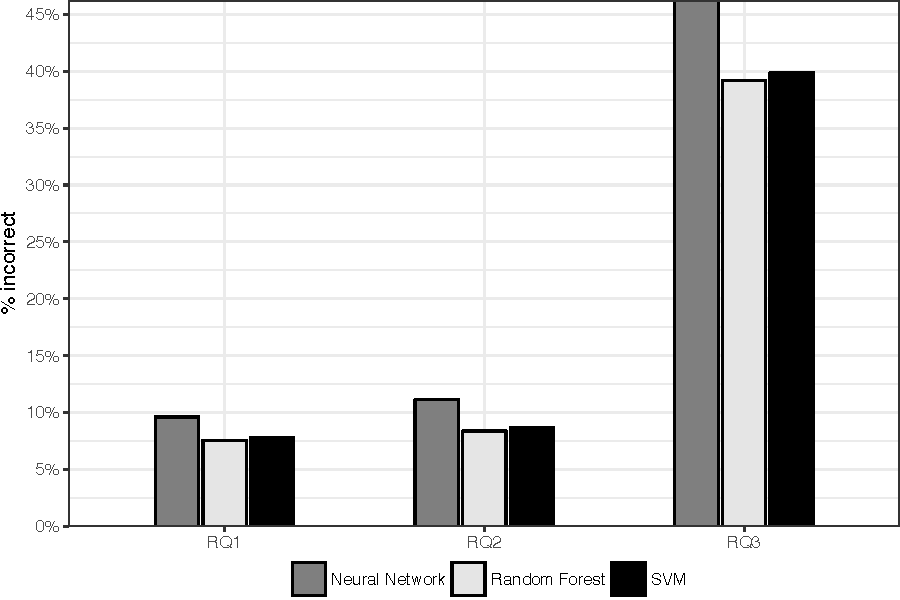
\includegraphics[scale=1]{figures/classifiers_performance_on_q1q2q3.pdf}
  \caption{Performance of ML algorithms for RQ1 and RQ2.}
  \label{fig:classifiers_performance_on_q1q2q3}
\end{figure*}

\subsection{RQ2: Will the CR severity level increase, decrease or remain the same?}\label{subsec:rq2}

The RQ2 poses a problem more difficult than the previous question. It is a question with three possible responses related to severity level: it has decreased (class -1); it has remained (class 0); and it has increased (class 1). Tables \ref{tab:classifiers_precision_on_rq2}, \ref{tab:classifiers_recall_on_rq2}, and \ref{tab:classifiers_f_measure_on_rq2} shows the performance of the ML algorithms to predict the response to this issue. 

\begin{table}[!ht]
	\renewcommand{\arraystretch}{1.8}
	\caption{ML algorithms precision performance on RQ2.}
	\label{tab:classifiers_precision_on_rq2}
	\centering
	\begin{tabular}{l|c|c|c|c|}
		\cline{2-5}
		& Class & Neural Network & Random Forest & SVM\\
		\cline{1-5}	
		\multicolumn{5}{ |c| }{Precision}\\
		\cline{1-5} 
        \multicolumn{1}{ |c| }{\multirow{3}{*}{\rotatebox[origin=c]{90}{\scriptsize{Cassandra}}}} & -1 & 0.4393939 & 0.7435897 & 0.7631579\\
		\cline{2-5}
		\multicolumn{1}{ |c| }{} & 0 & 0.9523305 & 0.9565445 & 0.9546403\\
		\cline{2-5}
		\multicolumn{1}{ |c| }{} & 1 & 0.7333333 & 0.7428571 & 0.8214286\\
		\hline
		\multicolumn{1}{ |c| }{\multirow{3}{*}{\rotatebox[origin=c]{90}{\scriptsize{Hadoop}}}} & -1 & 0.2272727 & 0.5555556 & 0.5000000\\
		\cline{2-5}
		\multicolumn{1}{ |c| }{} & 0 & 0.9549266 & 0.9551084 & 0.9520653\\
		\cline{2-5}
		\multicolumn{1}{ |c| }{} & 1 & 0.6060606 & 0.7195122 & 0.8666667\\
        \hline
		\multicolumn{1}{ |c| }{\multirow{2}{*}{\rotatebox[origin=c]{90}{\scriptsize{Spark}}}} 	& -1 & 0.2500000 & 0.5925926 & 0.5769231\\
		\cline{2-5}
		\multicolumn{1}{ |c| }{} & 0 & 0.9119788 & 0.9303548 & 0.9157695\\
		\cline{2-5}
		\multicolumn{1}{ |c| }{} & 1 & 0.5555556 & 0.6689655 & 0.7977528\\
		\cline{1-5} 
		\multicolumn{1}{ |c| }{} & Average & 0.6256502 & 0.7627867 & 0.7942671\\
		\hline
	\end{tabular}
\end{table}

\begin{table}[!ht]
	\renewcommand{\arraystretch}{1.8}
	\caption{ML algorithms recall performance on RQ2.}
	\label{tab:classifiers_recall_on_rq2}
	\centering
	\begin{tabular}{l|c|c|c|c|}
		\cline{2-5}
		& Class & Neural Network & Random Forest & SVM\\
		\cline{1-5}	
		\multicolumn{5}{ |c| }{Recall}\\
		\cline{1-5} 
        \multicolumn{1}{ |c| }{\multirow{3}{*}{\rotatebox[origin=c]{90}{\scriptsize{Cassandra}}}} & -1 & 0.2989691 & 0.2989691 & 0.29896907\\
		\cline{2-5}
		\multicolumn{1}{ |c| }{} & 0 & 0.9819771 & 0.9978154 & 1.00000000\\
		\cline{2-5}
		\multicolumn{1}{ |c| }{} & 1 & 0.3928571 & 0.4642857 & 0.41071429\\
		\hline
		\multicolumn{1}{ |c| }{\multirow{3}{*}{\rotatebox[origin=c]{90}{\scriptsize{Hadoop}}}} & -1 & 0.1111111 & 0.1111111 & 0.08888889\\
		\cline{2-5}
		\multicolumn{1}{ |c| }{} & 0 & 0.9753747 & 0.9908994 & 0.99946467\\
		\cline{2-5}
		\multicolumn{1}{ |c| }{} & 1 & 0.5172414 & 0.5086207 & 0.44827586\\
        \hline
		\multicolumn{1}{ |c| }{\multirow{2}{*}{\rotatebox[origin=c]{90}{\scriptsize{Spark}}}} 	& -1 & 0.1500000 & 0.2000000 & 0.18750000\\
		\cline{2-5}
		\multicolumn{1}{ |c| }{} & 0 & 0.9516575 & 0.9779006 & 0.99861878\\
		\cline{2-5}
		\multicolumn{1}{ |c| }{} & 1 & 0.4518072 & 0.5843373 & 0.42771084\\
		\cline{1-5} 
		\multicolumn{1}{ |c| }{} & Average & 0.5367772 & 0.5704376 & 0.5400158\\
		\hline
	\end{tabular}
\end{table}

\begin{table}[!ht]
	\renewcommand{\arraystretch}{1.8}
	\caption{ML algorithms F-measure performance on RQ2.}
	\label{tab:classifiers_f_measure_on_rq2}
	\centering
	\begin{tabular}{l|c|c|c|c|}
		\cline{2-5}
		& Class & Neural Network & Random Forest & SVM\\
		\cline{1-5}	
		\multicolumn{5}{ |c| }{F-measure}\\
		\cline{1-5} 
        \multicolumn{1}{ |c| }{\multirow{3}{*}{\rotatebox[origin=c]{90}{\scriptsize{Cassandra}}}} & -1 & 0.3558282 & 0.4264706 & 0.4296296\\
		\cline{2-5}
		\multicolumn{1}{ |c| }{} & 0 & 0.9669266 & 0.9767442 & 0.9767938\\
		\cline{2-5}
		\multicolumn{1}{ |c| }{} & 1 & 0.5116279 & 0.5714286 & 0.5476190\\
		\hline
		\multicolumn{1}{ |c| }{\multirow{3}{*}{\rotatebox[origin=c]{90}{\scriptsize{Hadoop}}}} & -1 & 0.1492537 & 0.1851852 & 0.1509434\\
		\cline{2-5}
		\multicolumn{1}{ |c| }{} & 0 & 0.9650424 & 0.9726747 & 0.9751893\\
		\cline{2-5}
		\multicolumn{1}{ |c| }{} & 1 & 0.5581395 & 0.5959596 & 0.5909091\\
        \hline
		\multicolumn{1}{ |c| }{\multirow{2}{*}{\rotatebox[origin=c]{90}{\scriptsize{Spark}}}} 	& -1 & 0.1875000 & 0.2990654 & 0.2830189\\
		\cline{2-5}
		\multicolumn{1}{ |c| }{} & 0 & 0.9313957 & 0.9535354 & 0.5290023\\
		\cline{2-5}
		\multicolumn{1}{ |c| }{} & 1 & 0.4983389 & 0.6237942 & 0.5568627\\
		\cline{1-5} 
		\multicolumn{1}{ |c| }{} & Average & 0.5693392 & 0.6227619 & 0.6073741\\
		\hline
	\end{tabular}
\end{table}

We tested the ML algorithms with 4580 (20\% of 22901) CR. Only now, we have three predicting situations: 4154 haven't changed their severity level, 246 have increased their severity level, and 180 have decreased their severity level. We can observe in Tables \ref{tab:classifiers_precision_on_rq2}, \ref{tab:classifiers_recall_on_rq2} and  \ref{tab:classifiers_f_measure_on_rq2} which the ML algorithms also performed very closely as question 1. However, the Random Forest algorithm had also the best performance in two out of three measures.

Figure \ref{fig:classifiers_performance_on_q1q2q3} shows that the ML algorithms performance had the same pattern in RQ2, as compared to RQ1. 

\subsection{RQ3: What is the prediction for the final CR severity level?}\label{subsec:rq3}

The RQ3 is a problem much harder than other two. It is a question with five responses related to severity level: (1) trivial; (2) minor; (3) major; (4) critical; and (5) blocker. Tables \ref{tab:classifiers_precision_on_rq3}, \ref{tab:classifiers_precision_on_rq3} and \ref{tab:classifiers_precision_on_rq3} shows the performance of the ML algorithms to predict the response to this issue. 

\begin{table}[!ht]
	\renewcommand{\arraystretch}{1.8}
	\caption{ML algorithms precision performance on RQ3.}
	\label{tab:classifiers_precision_on_rq3}
	\centering
	\begin{tabular}{l|c|c|c|c|}
		\cline{2-5}
		& Class & Neural Network & Random Forest & SVM\\
		\cline{1-5}	
		\multicolumn{5}{ |c| }{Precision}\\
		\cline{1-5} 
        \multicolumn{1}{ |c| }{\multirow{5}{*}{\rotatebox[origin=c]{90}{\scriptsize{Cassandra}}}} & 1 & 0.4022989 & 0.6976744 & 0.5348837\\
		\cline{2-5}
		\multicolumn{1}{ |c| }{} & 2 & 0.5394737 & 0.6209440 & 0.7513966\\
		\cline{2-5}
		\multicolumn{1}{ |c| }{} & 3 & 0.6645221 & 0.6924959 & 0.6222510\\
		\cline{2-5}
		\multicolumn{1}{ |c| }{} & 4 & 0.4782609 & 1.0000000 & 1.0000000\\
		\cline{2-5}
		\multicolumn{1}{ |c| }{} & 5 & 0.6666667 & 1.0000000 & 1.0000000\\
		\hline
		\multicolumn{1}{ |c| }{\multirow{5}{*}{\rotatebox[origin=c]{90}{\scriptsize{Hadoop}}}} & 1 & 0.2000000 & 0.9333333 & 0.8750000\\
		\cline{2-5}
		\multicolumn{1}{ |c| }{} & 2 & 0.3964497 & 0.7433628 & 0.9452055\\
		\cline{2-5}
		\multicolumn{1}{ |c| }{} & 3 & 0.6668558 & 0.7057175 & 0.6960305\\
		\cline{2-5}
		\multicolumn{1}{ |c| }{} & 4 & 0.3333333 & 1.0000000 & 1.0000000\\
		\cline{2-5}
		\multicolumn{1}{ |c| }{} & 5 & 0.4032258 & 0.9204545 & 1.0000000\\
        \hline
		\multicolumn{1}{ |c| }{\multirow{5}{*}{\rotatebox[origin=c]{90}{\scriptsize{Spark}}}} 	& 1 & 0.1818182 & 0.7142857 & 0.8000000\\
		\cline{2-5}
		\multicolumn{1}{ |c| }{} & 2 & 0.3345070 & 0.4785276 & 0.8194444\\
		\cline{2-5}
		\multicolumn{1}{ |c| }{} & 3 & 0.6096892 & 0.6131657 & 0.5994532\\
		\cline{2-5}
		\multicolumn{1}{ |c| }{} & 4 & 0.4807692 & 0.9733333 & 0.9726027\\
		\cline{2-5}
		\multicolumn{1}{ |c| }{} & 5 & 0.3703704 & 0.7857143 & 0.9500000\\
		\cline{1-5} 
		\multicolumn{1}{ |c| }{} & Average & 0.4485493
 & 0.7919339 & 0.8377511 \\
		\hline
	\end{tabular}
\end{table}
%
\begin{table}[!ht]
	\renewcommand{\arraystretch}{1.8}
	\caption{ML algorithms recall performance on RQ3.}
	\label{tab:classifiers_recall_on_rq3}
	\centering
	\begin{tabular}{l|c|c|c|c|}
		\cline{2-5}
		
		& Class & Neural Network & Random Forest & SVM\\
		\cline{1-5}	
		\multicolumn{5}{ |c| }{Recall}\\
		\cline{1-5} 
        \multicolumn{1}{ |c| }{\multirow{5}{*}{\rotatebox[origin=c]{90}{\scriptsize{Cassandra}}}} & 1 & 0.2243589 & 0.1923077 & 0.1474359\\
		\cline{2-5}
		\multicolumn{1}{ |c| }{} & 2 & 0.5766526 & 0.5921238 & 0.3783404\\
		\cline{2-5}
		\multicolumn{1}{ |c| }{} & 3 & 0.7053658 & 0.8282927 & 0.9385366\\
		\cline{2-5}
		\multicolumn{1}{ |c| }{} & 4 & 0.3283582 & 0.4626866 & 0.4626866\\
		\cline{2-5}
		\multicolumn{1}{ |c| }{} & 5 & 0.0800000 & 0.2400000 & 0.2400000\\
		\hline
		\multicolumn{1}{ |c| }{\multirow{5}{*}{\rotatebox[origin=c]{90}{\scriptsize{Hadoop}}}} & 1 & 0.0131578 & 0.1842105 & 0.1842105\\
		\cline{2-5}
		\multicolumn{1}{ |c| }{} & 2 & 0.1850828 & 0.2320442 & 0.1906077\\
		\cline{2-5}
		\multicolumn{1}{ |c| }{} & 3 & 0.9136858 & 0.9790047 & 0.9953344\\
		\cline{2-5}
		\multicolumn{1}{ |c| }{} & 4 & 0.1265822 & 0.3544304 & 0.3417722\\
		\cline{2-5}
		\multicolumn{1}{ |c| }{} & 5 & 0.1111111 & 0.3600000 & 0.3244444\\
        \hline
		\multicolumn{1}{ |c| }{\multirow{5}{*}{\rotatebox[origin=c]{90}{\scriptsize{Spark}}}} 	& 1 & 0.0312500 & 0.0781250 & 0.0625000\\
		\cline{2-5}
		\multicolumn{1}{ |c| }{} & 2 & 0.2691218 & 0.2209632 & 0.1671388\\
		\cline{2-5}
		\multicolumn{1}{ |c| }{} & 3 & 0.7494382 & 0.9314607 & 0.9853933\\
		\cline{2-5}
		\multicolumn{1}{ |c| }{} & 4 & 0.3989361 & 0.3882979 & 0.3776596\\
		\cline{2-5}
		\multicolumn{1}{ |c| }{} & 5 & 0.2531645 & 0.2784810 & 0.2405063\\
		\cline{1-5} 
		\multicolumn{1}{ |c| }{} & Average & 0.3310844
 & 0.4214952 & 0.4024377 \\
		\hline
	\end{tabular}
\end{table}
%
\begin{table}[!ht]
	\renewcommand{\arraystretch}{1.8}
	\caption{ML algorithms F-measure performance on RQ3.}
	\label{tab:classifiers_f_measure_on_rq3}
	\centering
	\begin{tabular}{l|c|c|c|c|}
		\cline{2-5}
		
		& Class & Neural Network & Random Forest & SVM\\
		\cline{1-5}	
		\multicolumn{5}{ |c| }{F-measure}\\
		\cline{1-5} 
        \multicolumn{1}{ |c| }{\multirow{5}{*}{\rotatebox[origin=c]{90}{\scriptsize{Cassandra}}}} & 1 & 0.2880658 & 0.3015075 & 0.2311558\\
		\cline{2-5}
		\multicolumn{1}{ |c| }{} & 2 & 0.5574439 & 0.6061915 & 0.5032741\\
		\cline{2-5}
		\multicolumn{1}{ |c| }{} & 3 & 0.6843350 & 0.7543314 & 0.7483469\\
		\cline{2-5}
		\multicolumn{1}{ |c| }{} & 4 & 0.3893805 & 0.6326531 & 0.6326531\\
		\cline{2-5}
		\multicolumn{1}{ |c| }{} & 5 & 0.1428571 & 0.3870968 & 0.3870968\\
		\hline
		\multicolumn{1}{ |c| }{\multirow{5}{*}{\rotatebox[origin=c]{90}{\scriptsize{Hadoop}}}} & 1 & 0.0246913 & 0.3076923 & 0.3043478\\
		\cline{2-5}
		\multicolumn{1}{ |c| }{} & 2 & 0.2523540 & 0.3536842 & 0.3172414\\
		\cline{2-5}
		\multicolumn{1}{ |c| }{} & 3 & 0.7709973 & 0.8201954 & 0.8192000\\
		\cline{2-5}
		\multicolumn{1}{ |c| }{} & 4 & 0.1834862 & 0.5233645 & 0.5094340\\
		\cline{2-5}
		\multicolumn{1}{ |c| }{} & 5 & 0.1742160 & 0.5175719 & 0.4899329\\
        \hline
		\multicolumn{1}{ |c| }{\multirow{5}{*}{\rotatebox[origin=c]{90}{\scriptsize{Spark}}}} 	& 1 & 0.0533333 & 0.1408451 & 0.1159420\\
		\cline{2-5}
		\multicolumn{1}{ |c| }{} & 2 & 0.2982731 & 0.3023256 & 0.2776471\\
		\cline{2-5}
		\multicolumn{1}{ |c| }{} & 3 & 0.6723790 & 0.7395183 & 0.7454314\\
		\cline{2-5}
		\multicolumn{1}{ |c| }{} & 4 & 0.4360465 & 0.5551331 & 0.5440613\\
		\cline{2-5}
		\multicolumn{1}{ |c| }{} & 5 & 0.3007518 & 0.4112150 & 0.3838384\\
		\cline{1-5} 
		\multicolumn{1}{ |c| }{} & Average & 0.3485740
 & 0.4902217 & 0.4673068 \\
		\hline
	\end{tabular}
\end{table}

We tested the ML algorithms with 4580 (20\% of 22901) CRs. Only now, we have six predicting situations: 288 are trivial; 1218 are minor; 2470 are major; 259 are critical; 345 are a blocker. We can observe in the Table \ref{tab:classifiers_precision_on_rq3}, \ref{tab:classifiers_recall_on_rq3} and \ref{tab:classifiers_f_measure_on_rq3} which the ML algorithms also performed very closely as questions 1 and 2. As in the two previous questions, the Random Forest algorithm had also the best performance in two out of three measures.

Figure \ref{fig:classifiers_performance_on_q1q2q3} shows that the ML algorithms performance had the same pattern in RQ1 and RQ2, as compared to RQ3.

\subsection{RQ4: How ML predictions compare to user prediction?}\label{subsec:rq4}
We have compared ML algorithms predictions to user prediction in terms of error magnitude. Figure \ref{fig:classifiers_performance_for_q3} shows predictors versus user error magnitude in the assignment of severity level.  Figure \ref{fig:classifiers_performance_for_q4} analyzes how well the ML prediction performed with respect to user prediction: better (ML algorithm error absolute value was smaller than user prediction error), equals (ML algorithm error equals to user error) or worse (ML algorithm error greater than user error).  The data clearly show that the use of this type of software predictor results in no gain to the user. This conclusion could not be drawn simply knowing the value of the classic accuracy measurement for Neural Network (2426/4580 = 52.969\%), Random Forest (2762/4580 = 60.305\%), and SVM (2731/4580 = 59.628\%) (see Figure \ref{fig:classifiers_performance_for_q4}). It is worth mentioning that our findings are in the same order of magnitude as findings reported in the literature. Therefore, one cannot state with confidence whether the use of the reported ML approach will bring any  benefit, as compared to a simple educated guess by the user. On the contrary, there is evidence that predictions produced under these conditions are worse than user educated guess.

\begin{figure*}[!ht]
\centering
  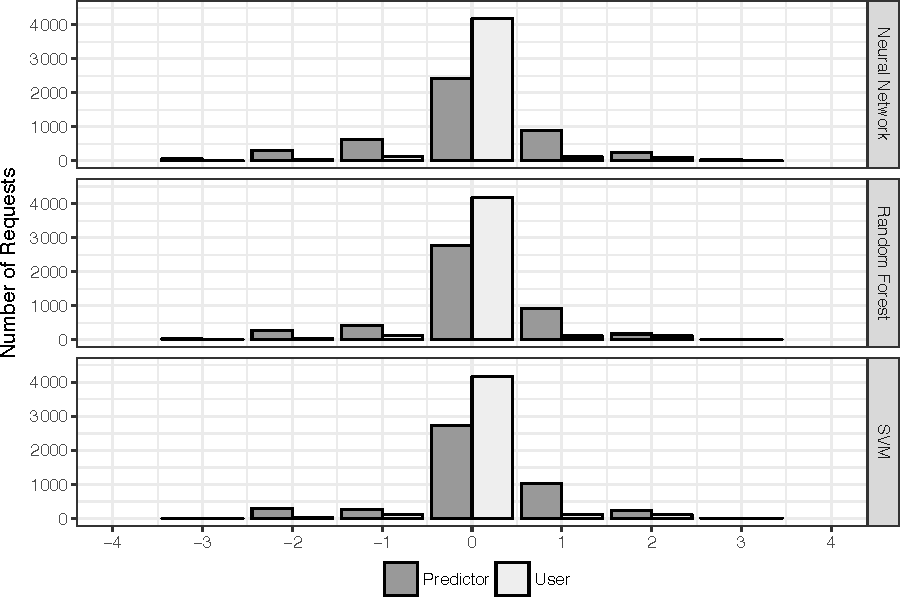
\includegraphics[scale=1]{figures/predictor_vs_user_error_magnitude.pdf}
  \caption{ML algorithms error magnitude (predictor versus user) for RQ3.}
    \label{fig:classifiers_performance_for_q3}
\end{figure*}

\begin{figure*}[!ht]
\centering
  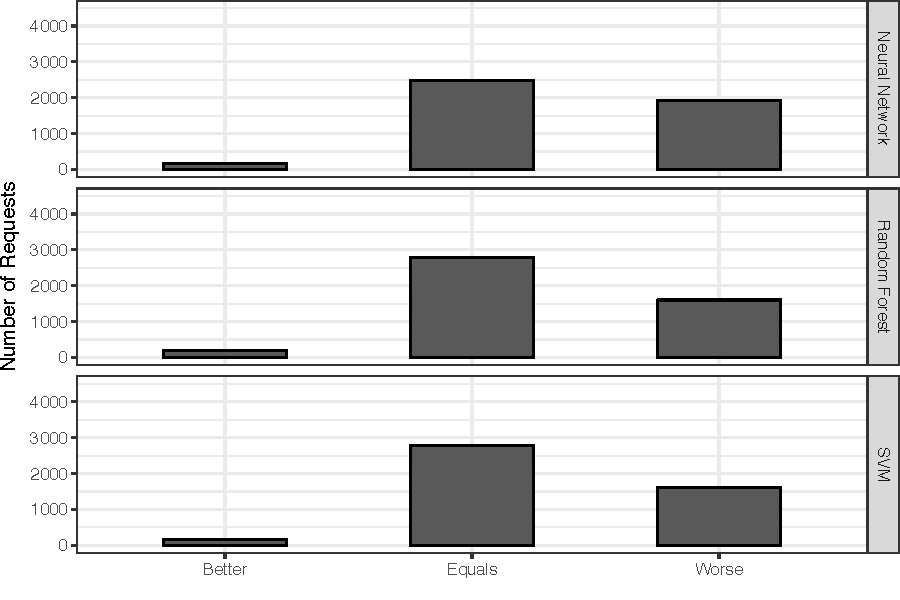
\includegraphics[scale=1]{figures/predictors_performance_compared_user.pdf}
  \caption{ML algorithms performance compared to user for RQ4.}
    \label{fig:classifiers_performance_for_q4}
\end{figure*}

\subsection{Statistical Tests}\label{subsec:tests}
We can one observe in the previous tables that the performance of the three ML algorithms are very similar. To confirm whether they are really similar, we have evaluated their F-measure performances using Friedman Test\cite{Japkowicz:2011}. 
We have defined the test null hypothesis (H0) as ``the investigated algorithms have similar performance``, and to test it, we have grouped F-measure values by dataset, research question and algorithm. For each group (3 per dataset), we have calculated the p-value.    Table \ref{tab:friedman_tests_results} shows the null hypothesis(H0) can be accepted (p$-$value $>=$ 0.05) to the most cases, confirming that the investigated algorithms are similar\cite{Demsar:2006}. 

\begin{table}[!ht]
	\renewcommand{\arraystretch}{1.8}
	\caption{Friedman tests results over F-measure.}
	\label{tab:friedman_tests_results}
	\centering
	\begin{tabular}{l|c|c|c|}
		\cline{2-4}
		
		& Question & P-value & H0\\
		\cline{1-4}
% Neural Network		
%		\multicolumn{5}{ |c| }{Neural Network}\\
%		\cline{1-5} 
        \multicolumn{1}{ |c| }{\multirow{3}{*}{\rotatebox[origin=c]{90}{\scriptsize{Cassandra}}}} & Q1 & 0.135335283 & Accepted\\
		\cline{2-4}
		\multicolumn{1}{ |c| }{} & Q2 & 0.096971968 & Accepted\\
		\cline{2-4}
        \multicolumn{1}{ |c| }{} & Q3 & 0.055637998 & Accepted\\
		\hline
		\multicolumn{1}{ |c| }{\multirow{3}{*}{\rotatebox[origin=c]{90}{\scriptsize{Hadoop}}}} & Q1 & 0.223130160 & Accepted\\
		\cline{2-4}
		\multicolumn{1}{ |c| }{} & Q2 & 0.096971968 & Accepted\\
		\cline{2-4}
		\multicolumn{1}{ |c| }{} & Q3 & 0.006737947 & Reject\\
		\hline
		\multicolumn{1}{ |c| }{\multirow{3}{*}{\rotatebox[origin=c]{90}{\scriptsize{Spark}}}} 		
		& Q1 & 0.223130160 & Accepted\\
		\cline{2-4}
		\multicolumn{1}{ |c| }{} & Q2 & 0.096971968 & Accepted\\
        \cline{2-4}
		\multicolumn{1}{ |c| }{} & Q3 & 0.040762204 & Reject\\
%		\cline{1-5} 
%		\multicolumn{1}{ |c| }{} & Average & 0.7988197 & 0.7057988 & 0.7404609\\
		\hline
	\end{tabular}
\end{table}

\subsection{Discussion}\label{subsec:discussion}

Table \ref{tab:performance_summary_literature} summarizes results related to CR severity level prediction reported in the literature and those generated during our experiments. We can observe that our results are better than others \cite{Lamkanfi2010, ValdiviaGarcia2014} to address RQ1 and RQ2. we can also note that our results are better than \cite{Tian2012} and worse than \cite{Menzies2008} to address RQ3. Notice that in many cases datasets and algorithms are different. 
\begin{table}[!h]
  \centering
  \renewcommand{\arraystretch}{1.7}
  \caption{ML algorithms performance summary (cells with a pair of numbers indicate range of variation).}
    \begin{tabular}{|c|p{2.1cm}|p{1.3cm}|c|p{1.8cm}|}
\cline{2-5}    \multicolumn{1}{r|}{} & \multicolumn{1}{c|}{Research Question} & \multicolumn{1}{c|}{Project} & F-measure & \multicolumn{1}{c|}{Algorithm} \\
    \hline
    \multirow{5}[10]{*}{\begin{turn}{88}\scriptsize{Menzies\cite{Menzies2008}}\end{turn}} & \multicolumn{1}{r|}{\multirow{5}[10]{2.1cm}{Is the bug report blocker, critical, major, minor or trivial?}} & PitsA & 14.0-17.0 & Ripper \\
\cline{3-5}          &       & PitsB & 42.0-90.0 & Ripper \\
\cline{3-5}          &       & PitsC & 53.0-92.0 & Ripper \\
\cline{3-5}          &       & PitsD & 87.0-99.0 & Ripper \\
\cline{3-5}          &       & PitsE & 8.0-88.0 & Ripper \\
    \hline
    \multirow{3}[6]{*}{\begin{turn}{88} $\quad$\scriptsize{Lamkanfi\cite{Lamkanfi2010}}\end{turn}} & \multicolumn{1}{r|}{\multirow{3}[6]{2.1cm}{Is the bug report severe or non-severe?}} & Mozilla & 65.9-71.7 & Naive Bayes \\
\cline{3-5}          &       & Eclipse & 62.5-65.5 & Naive Bayes \\
\cline{3-5}          &       & GNOME & 72.7-78.5 & Naive Bayes \\
    \hline
    \multirow{6}[12]{*}{\begin{turn}{88}\scriptsize{Valdivia\cite{ValdiviaGarcia2014}}\end{turn}} & \multicolumn{1}{r|}{\multirow{6}[12]{2.1cm}{Is the bug report blocking or non-blocking?}} & Chrominum & 15.3  & Decision Tree \\
\cline{3-5}          &       & Eclipse & 15.4  & Decision Tree \\
\cline{3-5}          &       & FreeDesktop & 31.9  & Decision Tree \\
\cline{3-5}          &       & Mozilla & 42.1  & Decision Tree \\
\cline{3-5}          &       & Netbeans & 21.1  & Decision Tree \\
\cline{3-5}          &       & Netbeans & 25.6  & Decision Tree \\
    \hline
    \multirow{3}[6]{*}{\begin{turn}{88}\scriptsize{Tian\cite{Tian2012}}\end{turn}} & \multicolumn{1}{r|}{\multirow{3}[6]{2.1cm}{Is the bug report blocker, critical, major, minor or trivial?}} & OpenOffice & 12.3-74.0 & INSPect \\
\cline{3-5}          &       & Mozilla & 13.9-65.3 & INSPect \\
\cline{3-5}          &       & Eclipse & 8.6-58.6 & INSPect \\
    \hline
    \multirow{9}[18]{*}{\begin{turn}{88}\scriptsize{Ours}\end{turn}} & \multicolumn{1}{r|}{\multirow{3}[6]{2.1cm}{Will the CR severity level change?}} & Cassandra & 65.50-97.88 & Random Forest \\
\cline{3-5}          &       & Hadoop & 53.16-97.09 & Random Forest \\
\cline{3-5}          &       & Spark & 64.15-94.87 & Random Forest \\
\cline{2-5}          & \multicolumn{1}{r|}{\multirow{3}[6]{2.1cm}{Will the CR severity level increase, decrease or remain the same?\linebreak$\quad$}} & Cassandra & 42.64-97.67 & Random Forest \\
\cline{3-5}          &       & Hadoop & 18.51-97.26 & Random Forest \\
\cline{3-5}          &       & Spark & 29.90-95.35 & Random Forest \\
\cline{2-5}          & \multicolumn{1}{r|}{\multirow{3}[6]{2.1cm}{Is the bug report blocker, critical, major, minor or trivial?}} & Cassandra & 30.15-75.43 & Random Forest \\
\cline{3-5}          &       & Hadoop & 30.76-82.01 & Random Forest \\
\cline{3-5}          &       & Spark & 14.08-73.95 & Random Forest \\
    \hline
    \end{tabular}%
  \label{tab:performance_summary_literature}%
\end{table}%  




